
\subsection{Shape Initialization}\label{sec:initialization}

\cxj{re-write this section. Describe clearly about the parameters, the objective, and methods. }

In this section we explain the reason why using a specific angle to each fold edge, and constructing our initialized model. The basic ideal is to interpret the folded state of a box as a series of rotation angles along each edge, and by setting specific value of angles which is $\pi/2$, we can have a rough model to assist the later optimization.
		
Observed from existing data in the Internet, most of the traditional cartons are cuboid, as the examples shown in Figure~\ref{fig:realdata} (a) and (b), they are used to put in files or delivering daily supplies. Although there is a recent trend to design more complicated layouts to attract consumers Figure~\ref{fig:realdata} (c), the shape of these unusual cartons is similar to orthogonality boxes as their functions are still packaging commodity. Based on this observation, we set $\pi/2$ as the value of rotation angle to each fold edge, and have the initialized model as Figure~\ref{fig:initial}.

As shown in Figure~\ref{fig:initial} (a), the traditional cartons as cuboid boxes can reach an ideal state, while the novel designs need a little refinement like the four examples in Figure~\ref{fig:initial} (b). Take the hexagonal box as an example, users only need to assign six paste faces into corresponding surface, the model of a feasible carton will be generated. As a result, we interactively allow users to add these constrains into our system and optimize to a desired model.

\begin{figure}
	\centering
	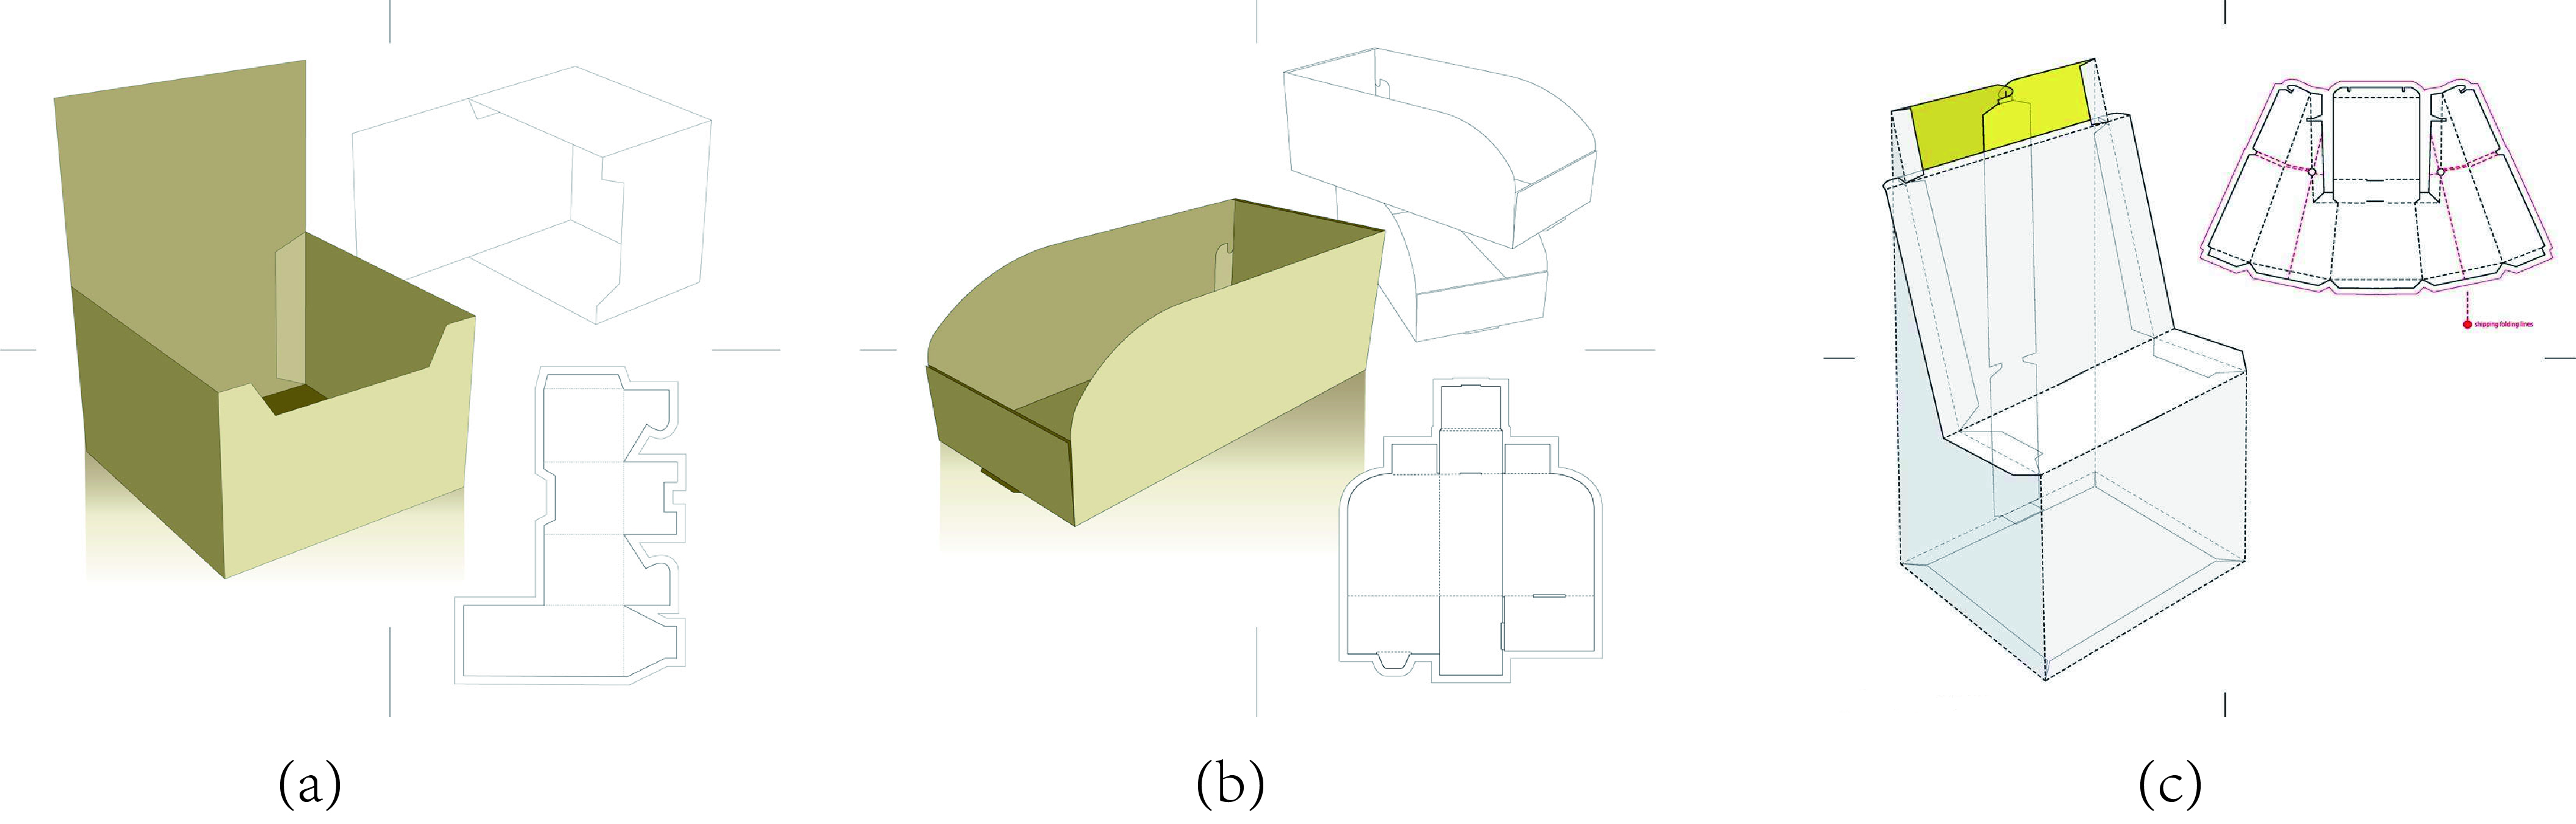
\includegraphics[width=0.9\textwidth]{images/realdata.jpg}
	\caption{Two traditional cartons (a), (b) and one unusual carton (c) with their corresponding layouts.}
	\label{fig:realdata}
\end{figure}

\begin{figure}
	\centering
	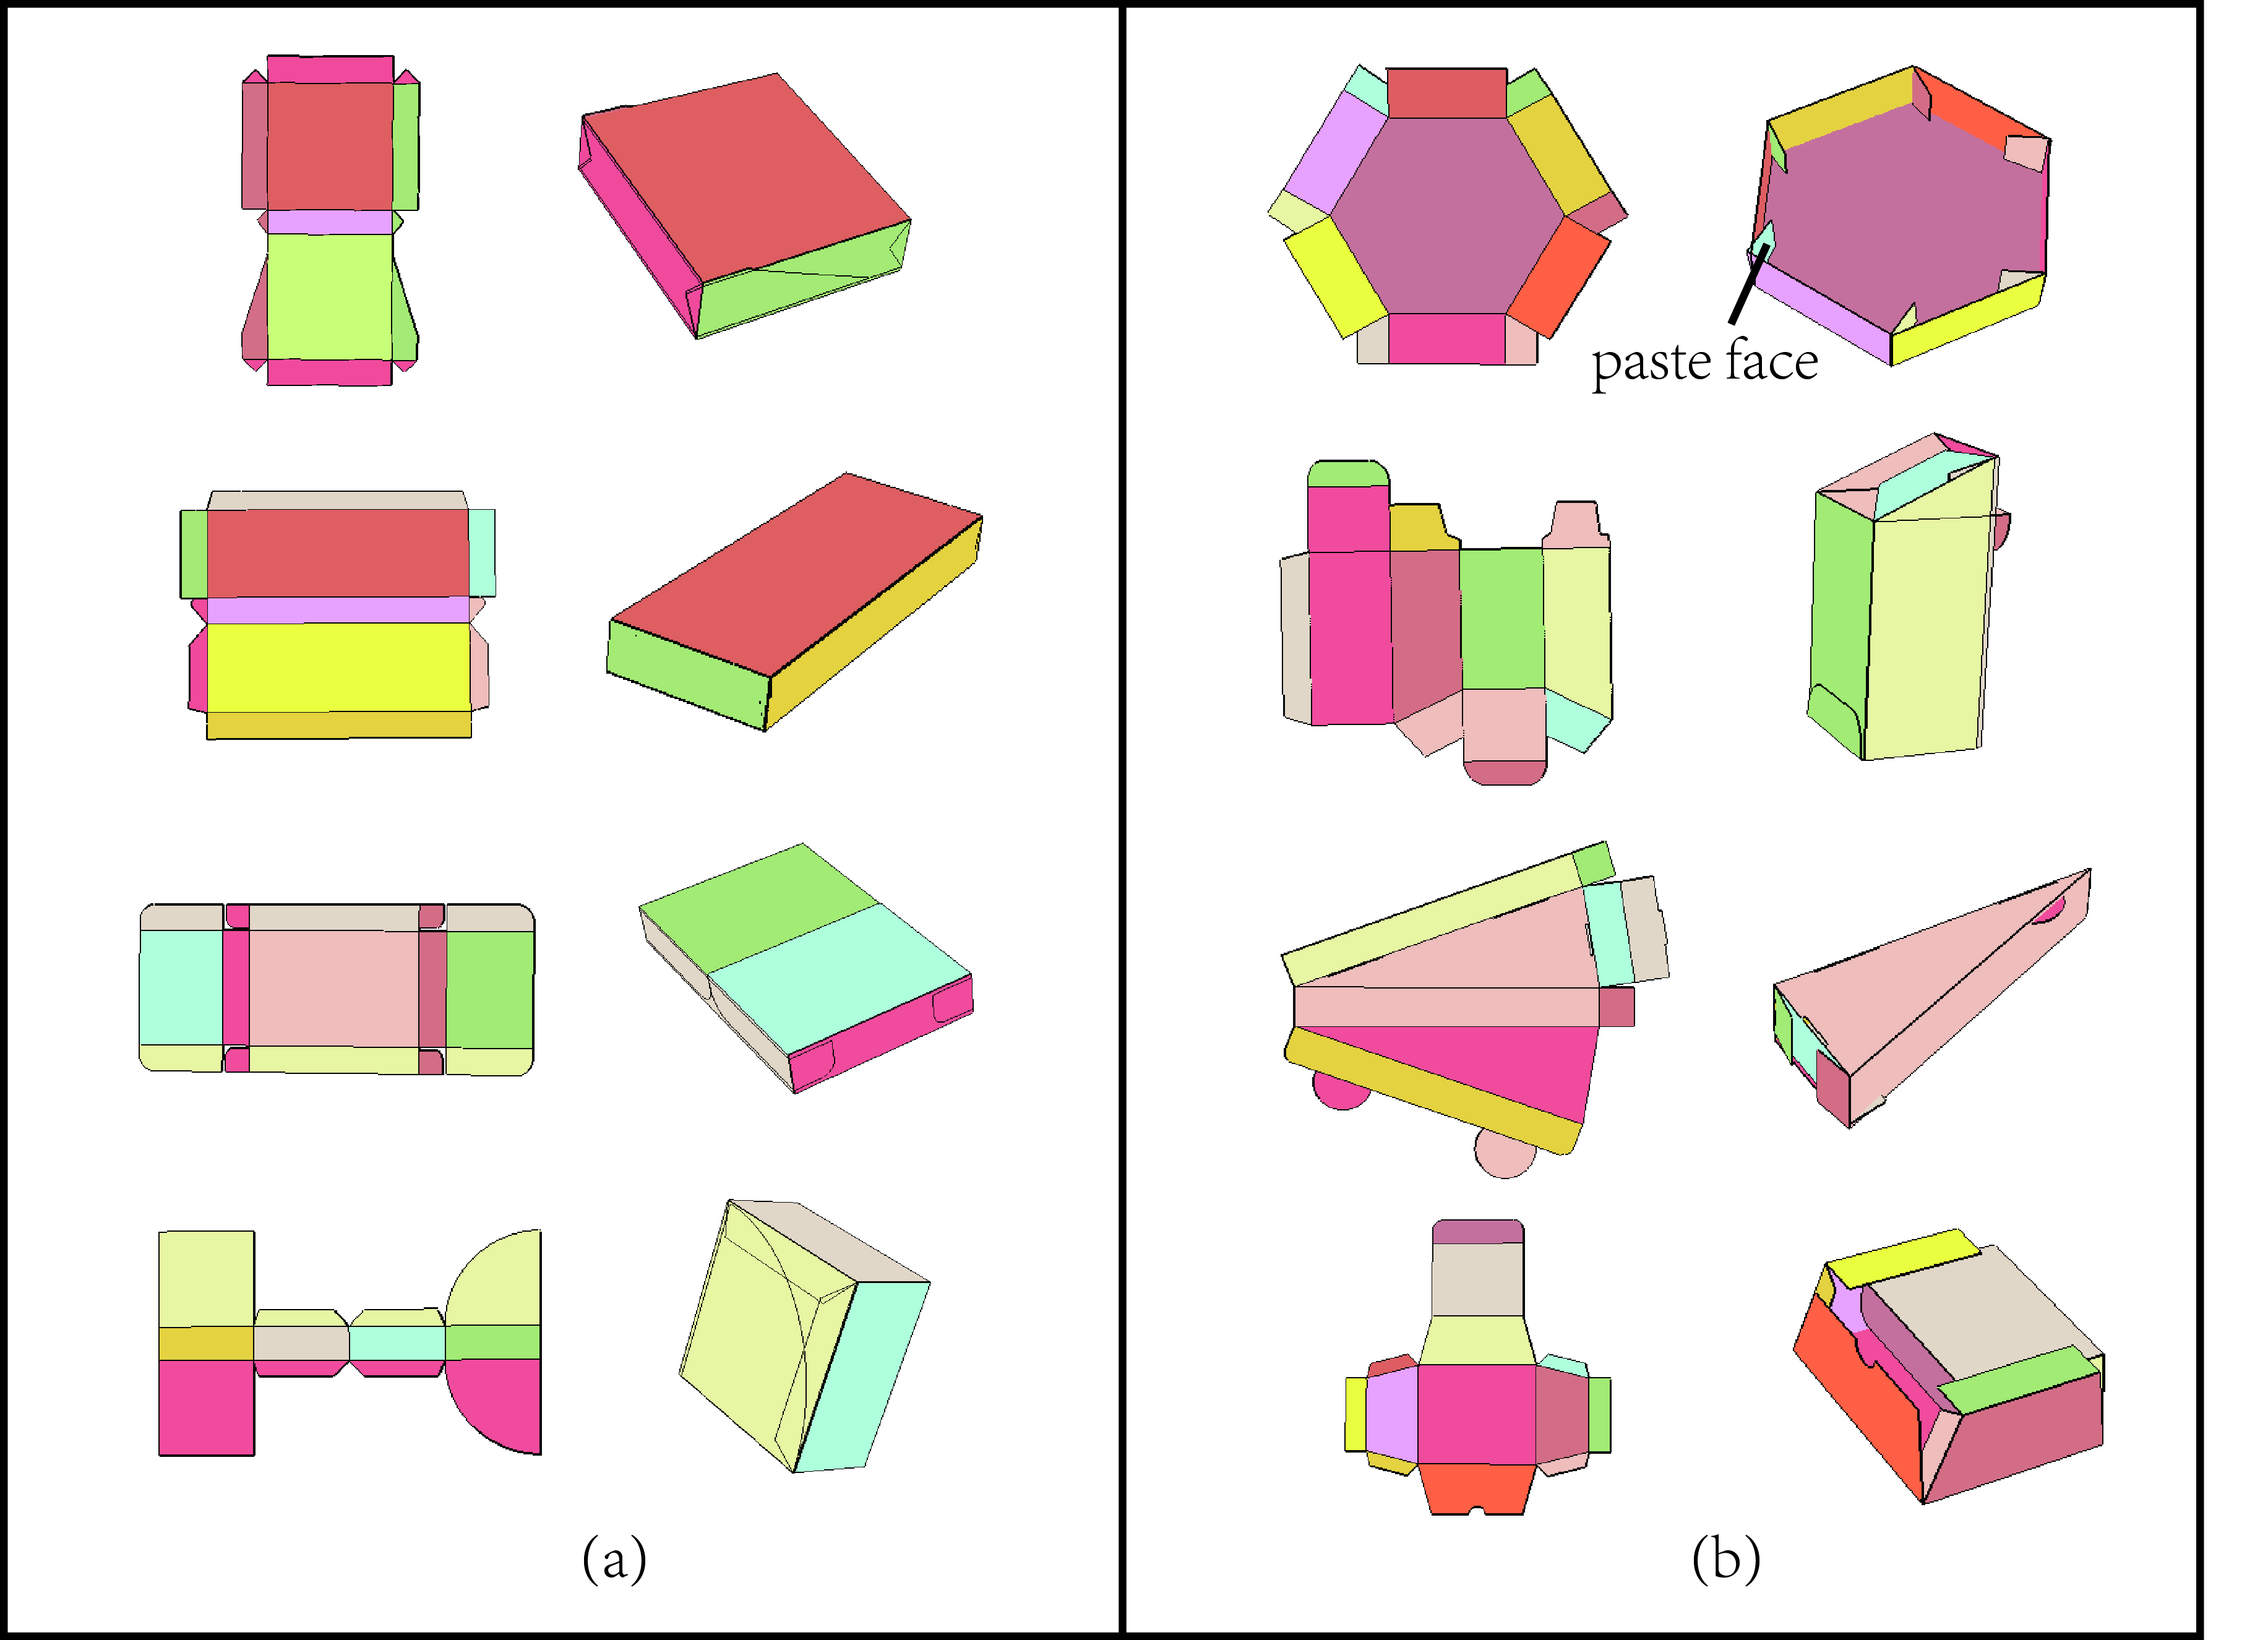
\includegraphics[width=0.9\textwidth]{images/initial.jpg}
	\caption{Eight different initialization results. Four initial cartons shown in the second column of (a) can reach the ideal state, the other four cartons need further refine (b).}
	\label{fig:initial}
\end{figure}

%%%%%%%%%%%%%%%%%%%%%%%%%%%%%%%%%%%%%%%%%%%%%%%%%%%%%%%%%%%%%%%%%%%%%
